%%%%%%%%%%%%%%%%%%%%%%%%%%%%%%%%%%%%%%%%%%%%%%%%%%%%%%%%%%%%%%%
%
% Welcome to Overleaf --- just edit your LaTeX on the left,
% and we'll compile it for you on the right. If you open the
% 'Share' menu, you can invite other users to edit at the same
% time. See www.overleaf.com/learn for more info. Enjoy!
%
%%%%%%%%%%%%%%%%%%%%%%%%%%%%%%%%%%%%%%%%%%%%%%%%%%%%%%%%%%%%%%%
\documentclass{beamer}
\usefonttheme[onlymath]{serif}
%Information to be included in the title page:
\title{Overview of TLS}
\author{Christopher Dickerman}
\date{05/01/24}

\begin{document}

\frame{\titlepage}

\begin{frame}
\frametitle{Overview of Presentation}
\begin{itemize}
    \item Theoretical Primitives
    \begin{itemize}
        \item Discrete Log Problem (DLP)
        \item Hidden Subgroup Problem (HSP)
        \item Finite Field Diffie-Hellman (DH)
        \item Elliptic Curve Diffie-Hellman (ECDH)
    \end{itemize}
    \item Implementation
    \begin{itemize}
        \item Certificates and Establishment of Trust
        \item Key Exchange
        \item Cipher Application Data
        \item Example TLS Handshake
    \end{itemize}
\end{itemize}
\end{frame}
\begin{frame}{Discrete Log Problem (DLP)}
    Consider the group $(\mathrm{G}, \cdot)$ with order $N$ and elements $\{e, g, g^2, g^3, ..., g^{N-1}\}$, where $g^k = \underbrace{g \cdot g \cdot ... \cdot g}_{k \text{ factors} }$ 
    \newline
    
    \textbf{The Discrete Log Problem}: Given some $x \in \mathrm{G}$, find the smallest $a$ such that $g^a = x$. This is denoted
    \[
        a = \log_{g}(x)
    \]
    
    The logarithm is only unique $\mathrm{mod}(N)$, since for any positive integer $k$,
    \[
        g^{a+k(N-1)} = g^{a}\cdot (g^{N-1})^k = g^a\cdot e = g^a
    \]
    
\end{frame}

\begin{frame}{Discrete Log Problem (DLP)}
\begin{itemize}
    \item Easy $\rightarrow$: Given $g$ and $a$, calculate $g^a = x$
    \begin{itemize}
        \item Naively $O(N)$, calculate $g^a$ by repeatedly multiplying $g$
        \item Better $O(\log(N))$, Precompute  $S = \{g, g^2, g^4, g^8, ..., g^{2^k}\}$, then $g^a$ is a sum of a subset of the elements of $S$
    \end{itemize}
        
    \item Hard $\leftarrow$: Given $g$ and $x$, calculate $\log_g{x} = a$
    \begin{itemize}
        \item Naively $O(N)$, calculate $g^k$ iterating $k$ until we get $x$
        \item Best achieved is $O(\sqrt{N})$, e.g. "Baby-step giant-step"
    \end{itemize}
\end{itemize}
    
\end{frame}

\begin{frame}{Hidden Subgroup Problem (HSP)}
    \begin{itemize}
        \item Prime factorization and the DLP are instances of the HSP
        \item Quantum algorithms can solve the HSP in polynomial time
    \end{itemize}
    \textbf{The Hidden Subgroup Problem}: Given a group $\mathrm{G}$, a subgroup $\mathrm{H}\leq \mathrm{G}$, and a set $\mathrm{X}$, we say a function $f:\mathrm{G} \rightarrow \mathrm{X}$ \textbf{hides} the subgroup $\mathrm{H}$ if 
    \[
            f(g_1) = f(g_2) \iff g_1\mathrm{H} = g_2\mathrm{H}, \forall g_1, g_2 \in \mathrm{G}
    \]

    
    Assume $f$ is an oracle and we don't know $\mathrm{H}$. The problem is to determine a generating set for $\mathrm{H}$ by using information gained by querying $f$.

\end{frame}

\begin{frame}{Hidden Subgroup Problem (HSP)}
    Example: 
    \begin{itemize}
        \item $\mathrm{G} = \mathbb{Z}_4, \mathrm{H} = \langle2\rangle, \mathrm{X} = \mathbb{Z}_4/\langle2\rangle$
        \item $f:\mathbb{Z}_4 \rightarrow \mathbb{Z}_4/\langle2\rangle$ where $ f(x) = x+ \{0, 2\}$
        \item We don't know anything besides $\mathrm{G}$, and we want to determine whether $\mathrm{H}$ is $\langle2\rangle$ or $\{0\}$.
        \item To solve, we can just naively check every element and see if the coset is equal to $f(0)$. If $f(0) = f(a)$, we know that $a\mathrm{H} = 0\mathrm{H} \implies a \in H$
        \begin{itemize}
            \item $f(0) = 0+\langle2\rangle = \{0, 2\}$
            \item $f(1) = 1+\langle2\rangle = \{1, 3\}$
            \item $f(2) = 2+\langle2\rangle = \{2, 0\} = \{0, 2\}$
            \item $f(3) = 3+\langle2\rangle = \{3, 1\} = \{1, 3\}$
        \end{itemize}
    \end{itemize}
    
\end{frame}

\begin{frame}{DLP as an Instance of HSP}
    Let $\mathrm{G} = \langle g\rangle, |\mathrm{G}| = N$. Given $x \in \mathrm{G}$, we want to obtain $\log_{g}(x)$.
    \\[10pt]
    We can represent this as a HSP in the group $\mathbb{Z}_N \times \mathbb{Z}_N$
    \\[10pt]
    Let $f:\mathbb{Z}_N \times \mathbb{Z}_N \rightarrow \mathrm{G}$, $f(a, b) = x^a g^b$
    \[
        f(a,b) = x^a g^b = g^{a \log_g(x) + b}
    \]
    
    Notice that $f$ is constant along lines 
    \[
        L_c = \{(a,b):a \log_g(x) + b = c \mod N \} 
    \]

    Each $L_c$ here is unique, that is if $c \neq c'$, then $L_c \neq L_{c'}$.


\end{frame}

\begin{frame}{DLP as an Instance of HSP}
    \[
        f(a,b) = x^a g^b = g^{a \log_g(x) + b}
    \]
    Here's what the sets $L_c$ look like:
    \[
        \scriptstyle L_c = \{(0, c), (1, -\log_g(x)+c), (2, -2\log_g(x)+c),... , (N - 1, -(N  - 1)\log_g(x)+c)\}
    \]
    And a set of particular interest to us is $L_0$:
    \[
        \scriptstyle L_0 = \{(0, 0), (1, -\log_g(x)), (2, -2\log_g(x)),... , (N - 1, -(N  - 1)\log_g(x))\}
    \]

    $\forall (a_0, b_0) \in L_0$, $f(a_0, b_0) = g^0 = 0$
    \begin{figure}
    \centering
    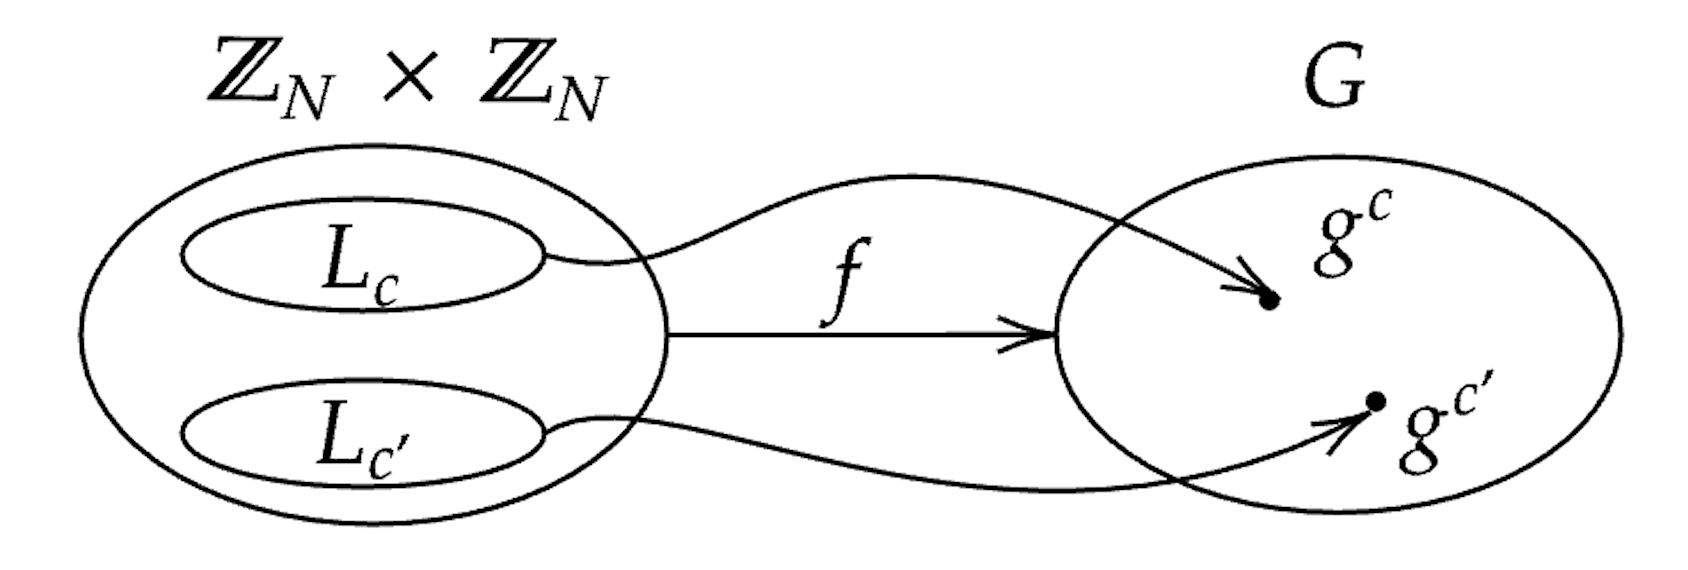
\includegraphics[width=0.6\linewidth]{figures/function diagram.png}
    \caption{A graphical representation of $f:\mathbb{Z}_N \times \mathbb{Z}_N \rightarrow \mathrm{G}$}
    \label{fig:enter-label}
\end{figure}
\end{frame}

\begin{frame}{DLP as an Instance of HSP}

    We can show that $f$ is a homomorphism:
    \[
    \begin{split}
        f((a_1, b_1)\oplus (a_2, b_2)) & = f(a_1+a_2, b_1+b_2) \\
         & = x^{a_1+a_2} g ^{b_1+b_2} \\
         & = x^{a_1} g^{b_1} x^{a_2} g^{b_2} \\
         & = f(a_1, b_1)f(a_2, b_2)
    \end{split}
    \]
    
    Notice that when $a \log_g(x) + b = 0$, $f(a,b) = 0$, so $\ker f = L_0$, and \[\frac{\mathbb{Z}_N \times \mathbb{Z}_N}{L_0} \cong G\] by the Fundamental Theorem on Homomorphisms
    
\end{frame}

\begin{frame}{DLP as an Instance of HSP}
    Given $\frac{\mathbb{Z}_N \times \mathbb{Z}_N}{L_0} \cong G$ and $f(a_1, b_1) = f(a_2,b_2)$, we have 
    \[(a_1, b_1)L_0 = (a_2,b_2)L_0\]
    \begin{figure}
        \centering
        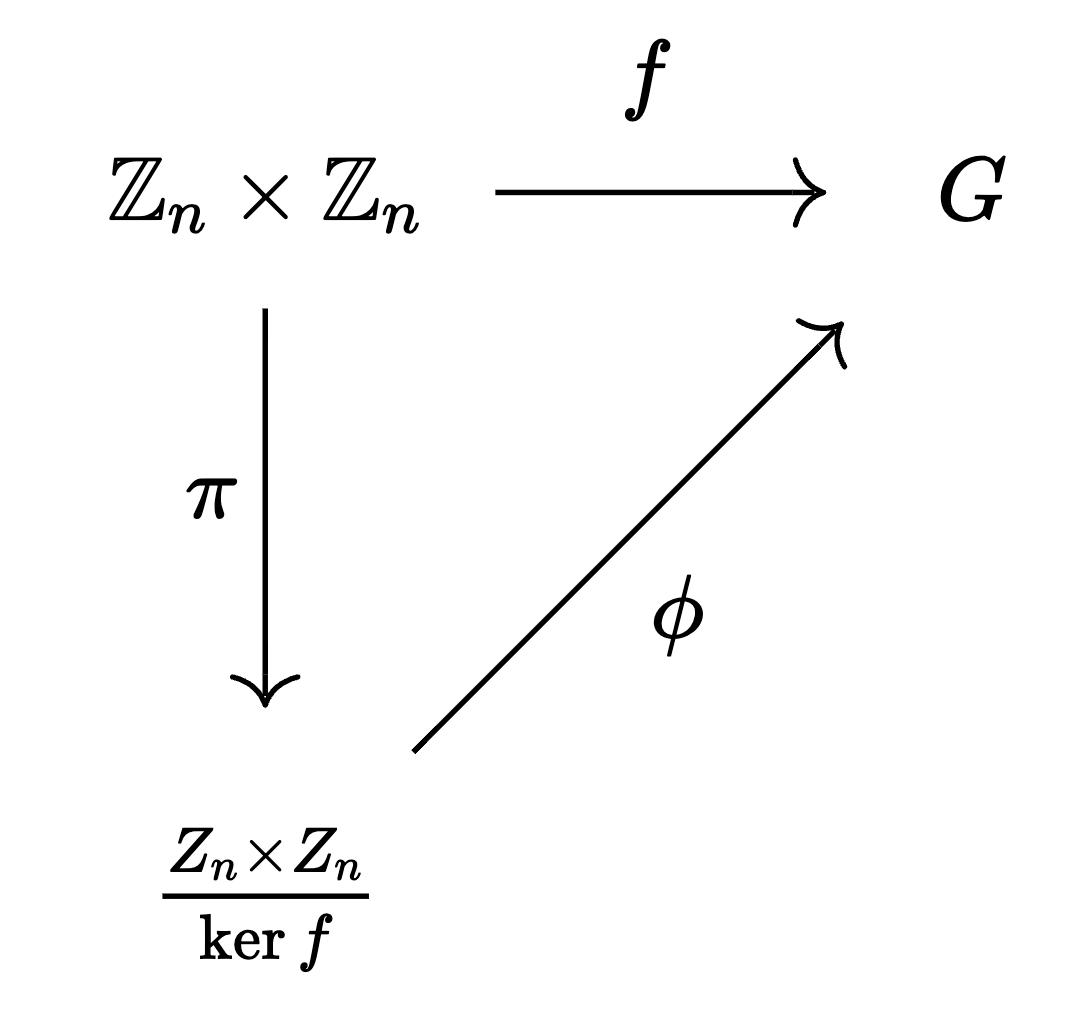
\includegraphics[width=0.4\linewidth]{figures/cd.png}
    \end{figure}
    Thus the construction yields a subgroup that reveals $\log_g(x)$ and satisfies the conditions of the Hidden Subgroup Problem.
\end{frame}

\begin{frame}{Finite Field Diffie-Hellman (DH)}
    Alice and Bob want to share a secret without an eavesdropper Eve being able to see that secret. Alice chooses a large prime $p$ and a number $g \in \mathbb{F^*}_p$. She sends this to Bob.

    Then 
    \begin{itemize}
        \item Alice:
        \begin{itemize}
            \item Chooses a secret $a \in \mathbb{F^*}_p$
            \item Computes $A = g^a$ and sends it to Bob
            \item Receives $B$ and computes $B^a=(g^{b})^{a}=g^{ab}$ 
        \end{itemize}
        \item Bob:
        \begin{itemize}
            \item Chooses a secret $b \in \mathbb{F^*}_p$
            \item Computes $B = g^b$ and sends it to Alice
            \item Receives $A$ and computes $A^b=(g^{a})^{b}=g^{ab}$
        \end{itemize}
        \item Eve:
        \begin{itemize}
            \item Receives $A=g^a$
            \item Receives $B=g^b$
            \item Attempts to compute $g^{ab}$
        \end{itemize}
    \end{itemize}

\end{frame}

\begin{frame}{Elliptic Curve Diffie-Hellman (ECDH)}
    Elliptic curves are curves in $\mathbb{R}^2$ satisfying the equation
    \[
        y^2 = x^3 + Ax + B
    \]

    We can define a notion of "addition" on the points of a elliptic curve for points $P$ and $Q$. To compute $P \oplus Q$, create the line $PQ$. If $PQ$ intersects the curve on a point not $P$ or $Q$, call that point $R$. Then $P \oplus Q = - R$, otherwise $P \oplus Q = O$, where $O$ is a point at infinity, and also the identity element.
    \begin{figure}
        \centering
        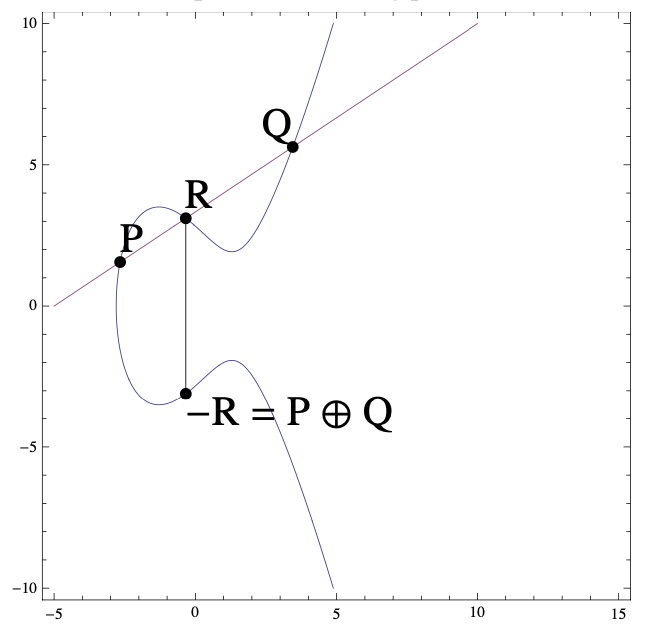
\includegraphics[width=0.3\linewidth]{figures/ec_addition.png}
        \caption{Elliptic curve "addition".}
        \label{fig:enter-label}
    \end{figure}

    
\end{frame}

\begin{frame}{Elliptic Curve Diffie-Hellman (ECDH)}
    This construction satisfies the following algebraic properties:
    \[
    \begin{split}
        \scriptstyle P \oplus Q & \scriptstyle = Q \oplus P \\
        \scriptstyle P \oplus O & \scriptstyle = P \\
        \scriptstyle P \oplus (Q \oplus R) & \scriptstyle = (P \oplus Q) \oplus R \\
        \scriptstyle P \oplus (-P) & \scriptstyle = O \\
    \end{split}
    \]
    And it gives us the following special rules:
    \[
    \begin{split}
        \scriptstyle \text{If } P \neq Q \text{ and } x_1 = x_2 \text{: } P \oplus Q & \scriptstyle = O \\
        \scriptstyle \text{If } P = Q \text{ and } y_1 = y_2 \text{: } P \oplus Q & \scriptstyle = O \\
        \scriptstyle \text{Otherwise: } P \oplus Q & \scriptstyle {= (m^2 - x_1 - x_2, -m^3+m(x_1+x_2)-b)}
    \end{split}
    \]

    {\scriptsize With $P = (x1, y_1)$, $Q = (x_2, y_2)$, $m = \frac{y_2 - y_1}{x_2 - x_1}$ and $b = y_1 - mx_1$}
\end{frame}

\begin{frame}{Elliptic Curve Diffie-Hellman (ECDH)}
    \[
         P \oplus Q = (m^2 - x_1 - x_2, -m^3+m(x_1+x_2)-b)
    \]
    \[
        m = \frac{y_2 - y_1}{x_2 - x_1} \text{ and } b = y_1 - mx_1
    \]
    When calculating on a finite field $\mathbb{F^*}_p$, we need to find $\frac{1}{x_2-x_1}$ to calculate $m$. Fractions aren't allowed but given a value $a$ we can find $a^{-1}$. By Fermat's Last Theorem:
    \[
        a^{p-1} \equiv 1 \text{ } \mathrm{mod}(p)
    \]
    So $a^{-1} = a^{p - 2}$
\end{frame}

\begin{frame}{Elliptic Curve Diffie-Hellman (ECDH)}
    In the group of $E(\mathbb{F}_p)$ of an elliptic curve over a finite field generated by $P$, we can define repeated addition:
    \[
        n\cdot P = \underbrace{P \oplus P \oplus \cdots \oplus P}_{n \text{ times} }
    \]

    \textbf{The Elliptic Curve Discrete Log Problem}: Given some $x \in E(\mathbb{F}_p)$, find the smallest $a$ such that 
    \[
        a\cdot P = x
    \]
\end{frame}

\begin{frame}{Elliptic Curve Diffie-Hellman (ECDH)}
    Alice and Bob want to share a secret without an eavesdropper Eve being able to see that secret. Alice chooses a large prime $p$ and a point $P \in E(\mathbb{F^*}_p)$. She sends this to Bob.

    Then 
    \begin{itemize}
        \item Alice:
        \begin{itemize}
            \item Chooses a secret $a \in E(\mathbb{F^*}_p)$
            \item Computes $A = a \cdot P$ and sends it to Bob
            \item Receives $B$ and computes $a \cdot B=a \cdot (b\cdot P) = ab \cdot P$
        \end{itemize}
        \item Bob:
        \begin{itemize}
            \item Chooses a secret $b \in E(\mathbb{F^*}_p)$
            \item Computes $B = b \cdot P$ and sends it to Alice
            \item Receives $A$ and computes $b \cdot A=b \cdot (a\cdot P) = ab \cdot P$
        \end{itemize}
        \item Eve:
        \begin{itemize}
            \item Receives $A=a \cdot P$
            \item Receives $B=b \cdot P$
            \item Attempts to compute $ab \cdot P$
        \end{itemize}
    \end{itemize}
\end{frame}

\begin{frame}{TLS}
    TLS itself can be broken down into 2 parts, from the \href{https://www.rfc-editor.org/rfc/rfc8446.txt}{specification}.
    \begin{itemize}
        \item "A handshake protocol that authenticates the
        communicating parties, negotiates cryptographic modes and
        parameters, and establishes shared keying material."

        \item "A record protocol that uses the parameters established
        by the handshake protocol to protect traffic between the
        communicating peers."
    \end{itemize}
\end{frame}

\begin{frame}{TLS Handshake: Certificates}
    \begin{itemize}
        \item I know I'm securely talking to someone, but how do I know who that is?
        \item MITM attack where Eve relays between Alice and Bob, supplying each with her public key $E$.
        \item Ideally we'd like some correspondence between real world entities and network entities that we can verify.
    \end{itemize}
\end{frame}

\begin{frame}{Digital Signature Algorithms}
    Samantha wants to approve some document $D$ and provide information (signature) $D^{\text{sig}}$, so that given $D$ and $D^{\text{sig}}$, Victor can verify Samantha's approval. We can use the tools of asymmetric cryptography to do this.
    \begin{figure}
        \centering
        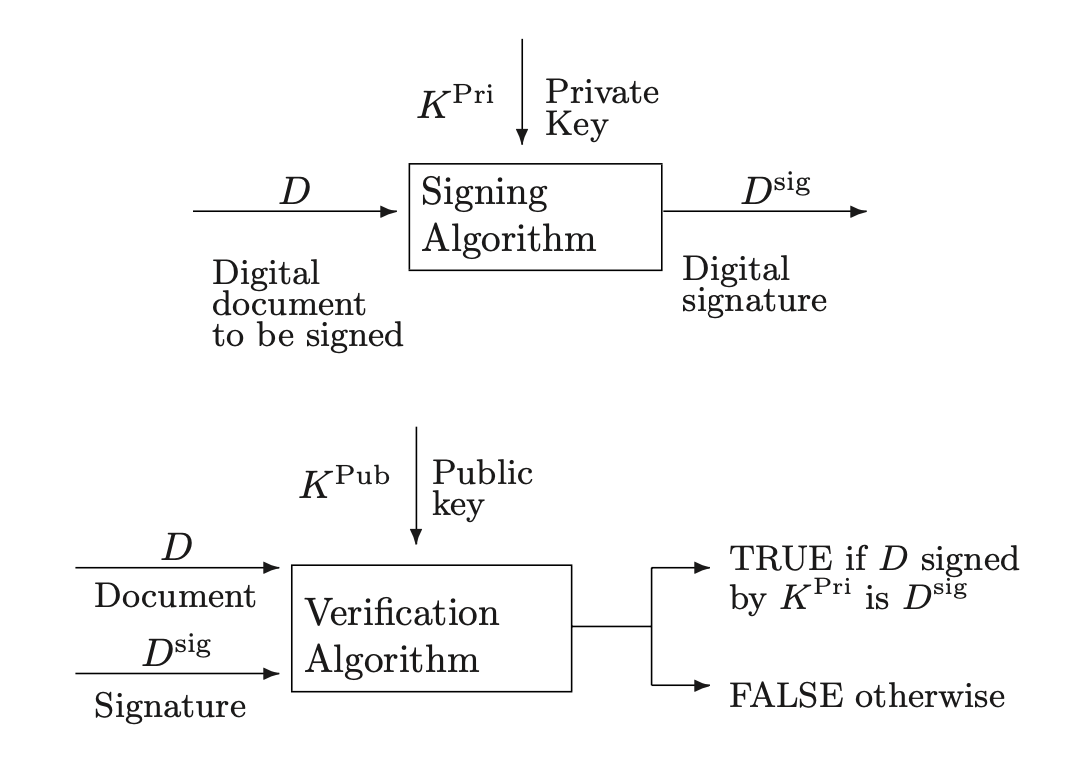
\includegraphics[width=0.7\linewidth]{figures/DSA.png} 
    \end{figure}
\end{frame}

\begin{frame}{RSA Digital Signature Algorithm}
    \textbf{Euler's Formula for pq}:
    If $p$ and $q$ are distinct primes and $\gcd(a,pq) = 1$
    \[a^{(p-1)(q-1)} \equiv 1 \mod pq\]

    Proof: 
    Start with showing that it is congruent modulo $p$
    \[ \left( a^{(p-1)}\right)^{(q-1)} \equiv 1^{(q-1)} \mod p\]
    \[1^{(q-1)} \equiv 1 \mod p \]
    Now showing that it is congruent modulo $q$
    \[ \left( a^{(q-1)}\right)^{(p-1)} \equiv 1^{(p-1)} \mod q\]
    \[1^{(p-1)} \equiv 1 \mod q \]
\end{frame}

\begin{frame}{RSA Digital Signature Algorithm}
    \[\implies p \text{ } | \left( a^{(p-1)(q-1)} - 1 \right) \text{  and }  q \text{ } |\left( a^{(p-1)(q-1)} - 1 \right)\]
    \[\implies pq \text{ } | \left( a^{(p-1)(q-1)} - 1 \right) \]
    \[\implies a^{(p-1)(q-1)} \equiv 1 \mod pq \]
    
    If we add $1$ to the exponent then we get
    \[a^{(p-1)(q-1) + 1} \equiv a \mod pq\]

    If we have some $s$ such that $\gcd(s, (p-1)(q-1)) = 1$, then there is an inverse which is to say there is some $v$ and $k$ such that
    \[ sv \equiv 1  \mod(p-1)(q-1)\]
    \[\implies a^{sv} \equiv a^{1 + k(p-1)(q-1)} \equiv a \mod pq \]
    
\end{frame}

\begin{frame}{RSA Digital Signature Algorithm}
    \[ sv \equiv 1 \mod(p-1)(q-1)\]
    Now if we have some document $D$ we want to authenticate, we can sign it with
    \[S \equiv D^{s} \mod pq\]
    And call $S$ the signature, then we can verify this signature with $v$ and get the document back
    \[S^{v} \equiv D^{sv} \equiv D \mod pq\]
\end{frame}

\begin{frame}{RSA Digital Signature Algorithm}
    Victor wants to make sure that a document $D$ has been signed by Samantha and that it hasn't been forged. Samantha chooses two large primes $p$ and $q$ with $pq = N$ and some verification exponent with $\gcd(v, (p-1)(q-1)) = 1$. She publishes $(N, v)$. Then she calculates $s$ that satisfies $sv \equiv 1 \mod((p-1)(q-1))$
    
    \begin{itemize}
        \item Samantha:
        \begin{itemize}
            \item Calculates $S \equiv D^s \mod(pq)$ and sends it to Victor
        \end{itemize}
        \item Victor:
        \begin{itemize}
            \item Receives $S$ and computes $S^{v} \equiv D^{sv} \equiv D \mod N$
        \end{itemize}
    \end{itemize}
\end{frame}

\begin{frame}{TLS Handshake: Certificates}
    We can use the RSA signature algorithm to make sure a site is who they say they are. Looking at google.com shows us they are using PKCS \#1 SHA-256 With RSA Encryption
    \begin{figure}
        \centering
        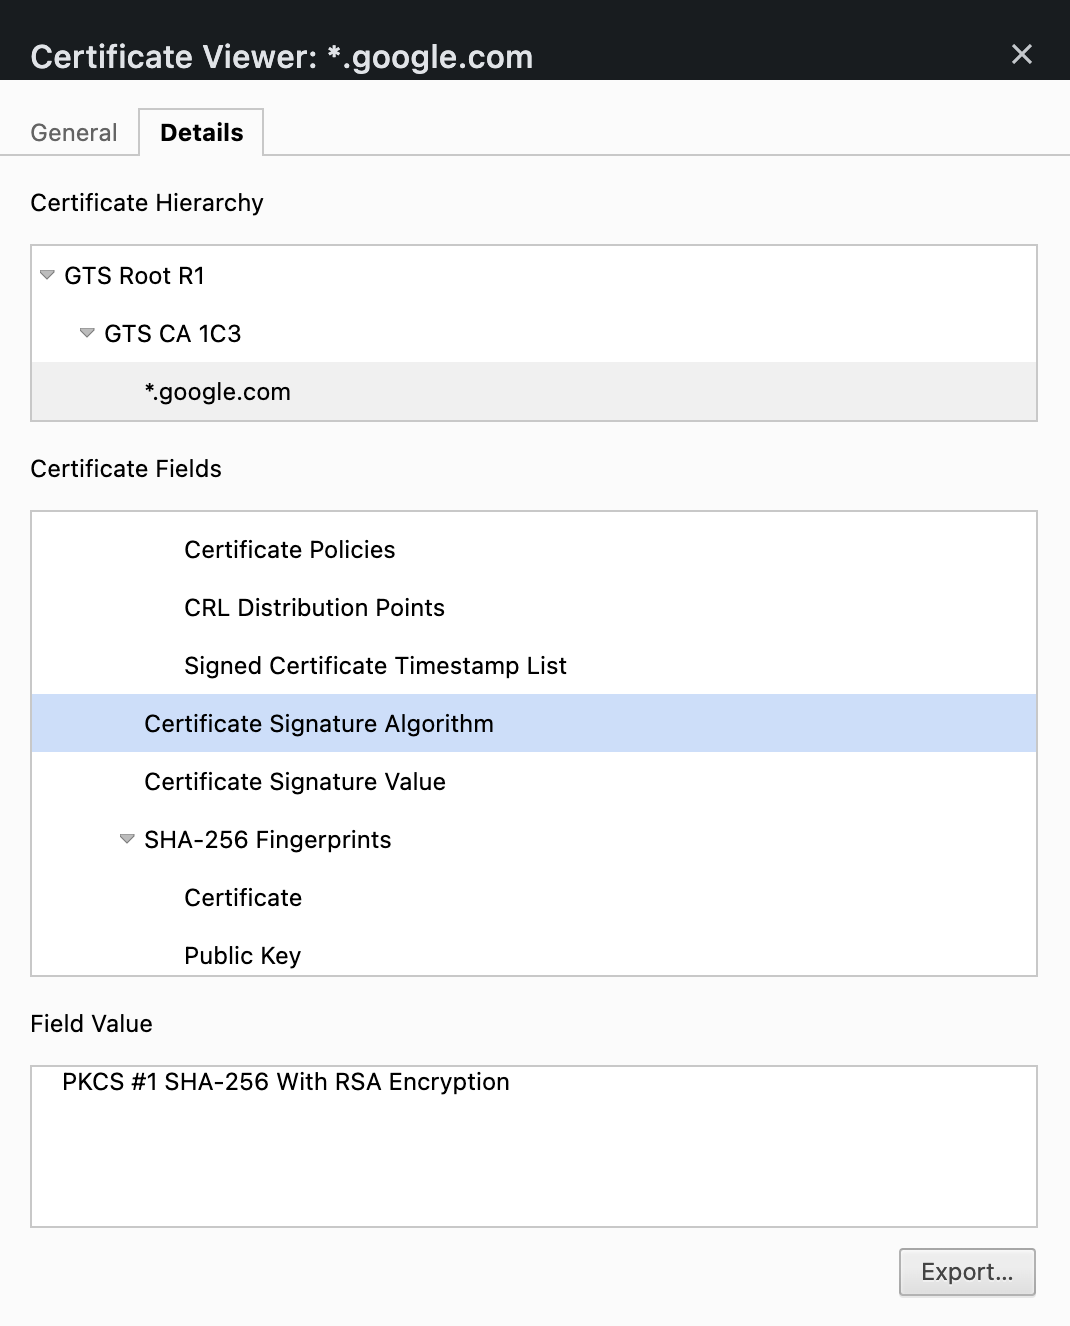
\includegraphics[width=0.35\linewidth]{figures/google certificate.png}
    \end{figure}
    \begin{itemize}
        \item Root certificates are stored in browser
        \item Certificate authorities can grant further certificates
        \item This builds a hierarchy of trust
    \end{itemize}
\end{frame}

\begin{frame}{TLS Handshake}
    Now that we can know who we are talking to, we can begin the TLS handshake.
    \begin{figure}
        \centering
        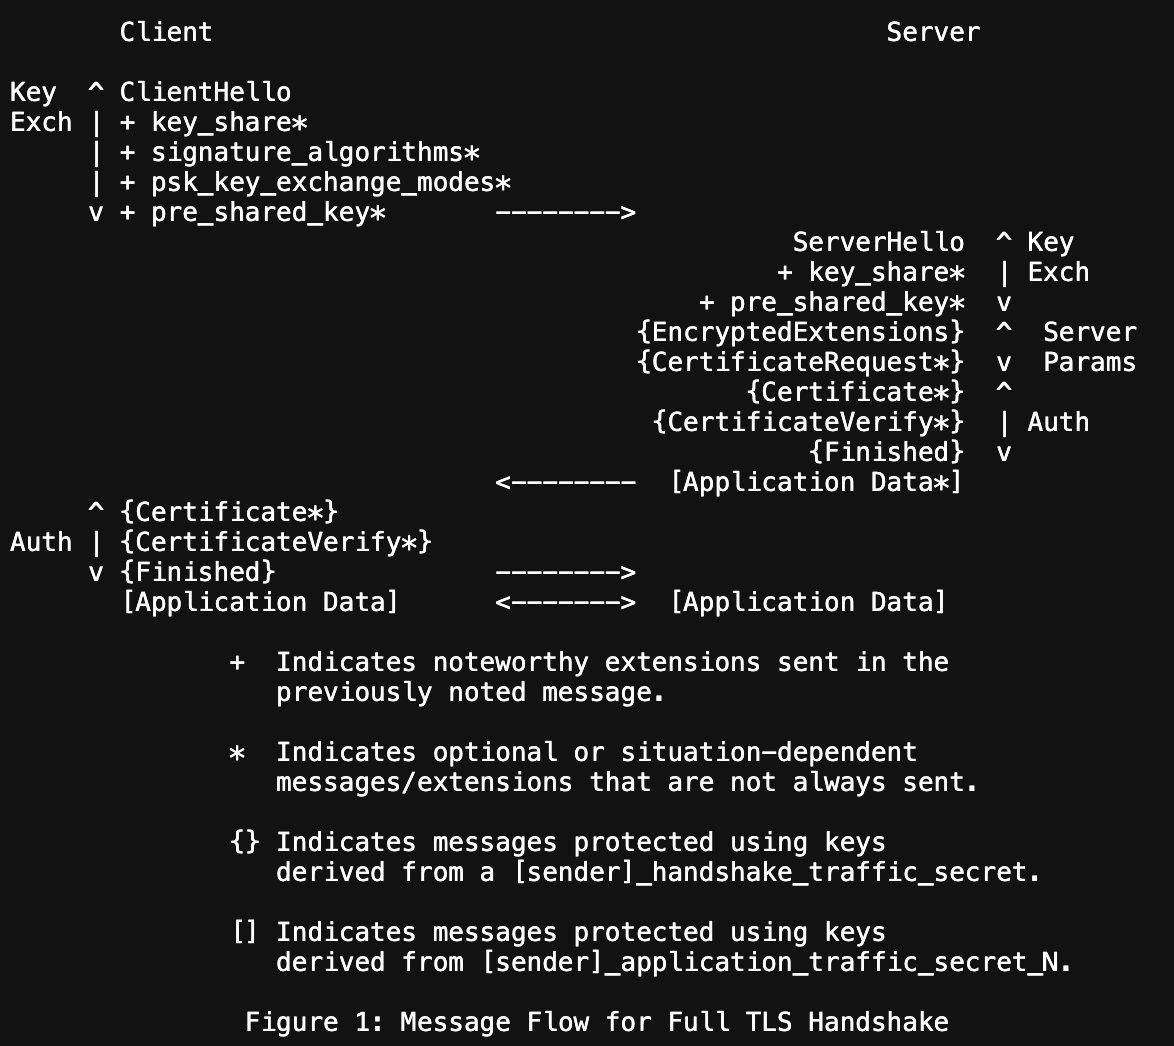
\includegraphics[width=.5\textwidth]{figures/handshake.png}
    \end{figure}
    \begin{figure}
        \centering
        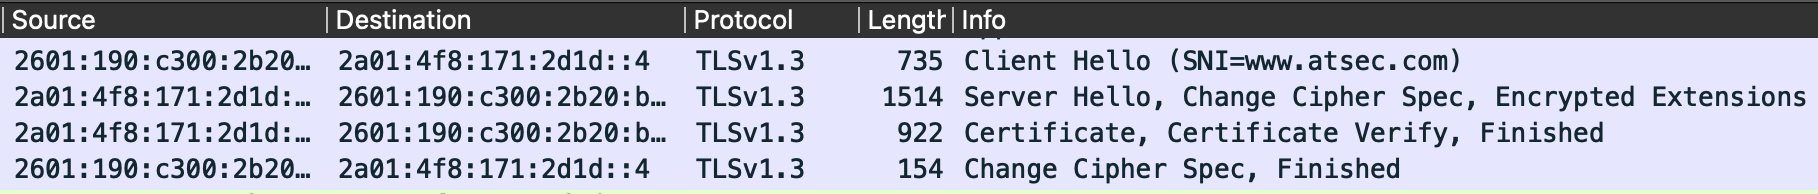
\includegraphics[width=.6\textwidth]{figures/real_hs.png}
    \end{figure}
\end{frame}

\begin{frame}{TLS Handshake: clientHello}
    We begin with the \texttt{clientHello}
    \begin{figure}
        \centering
        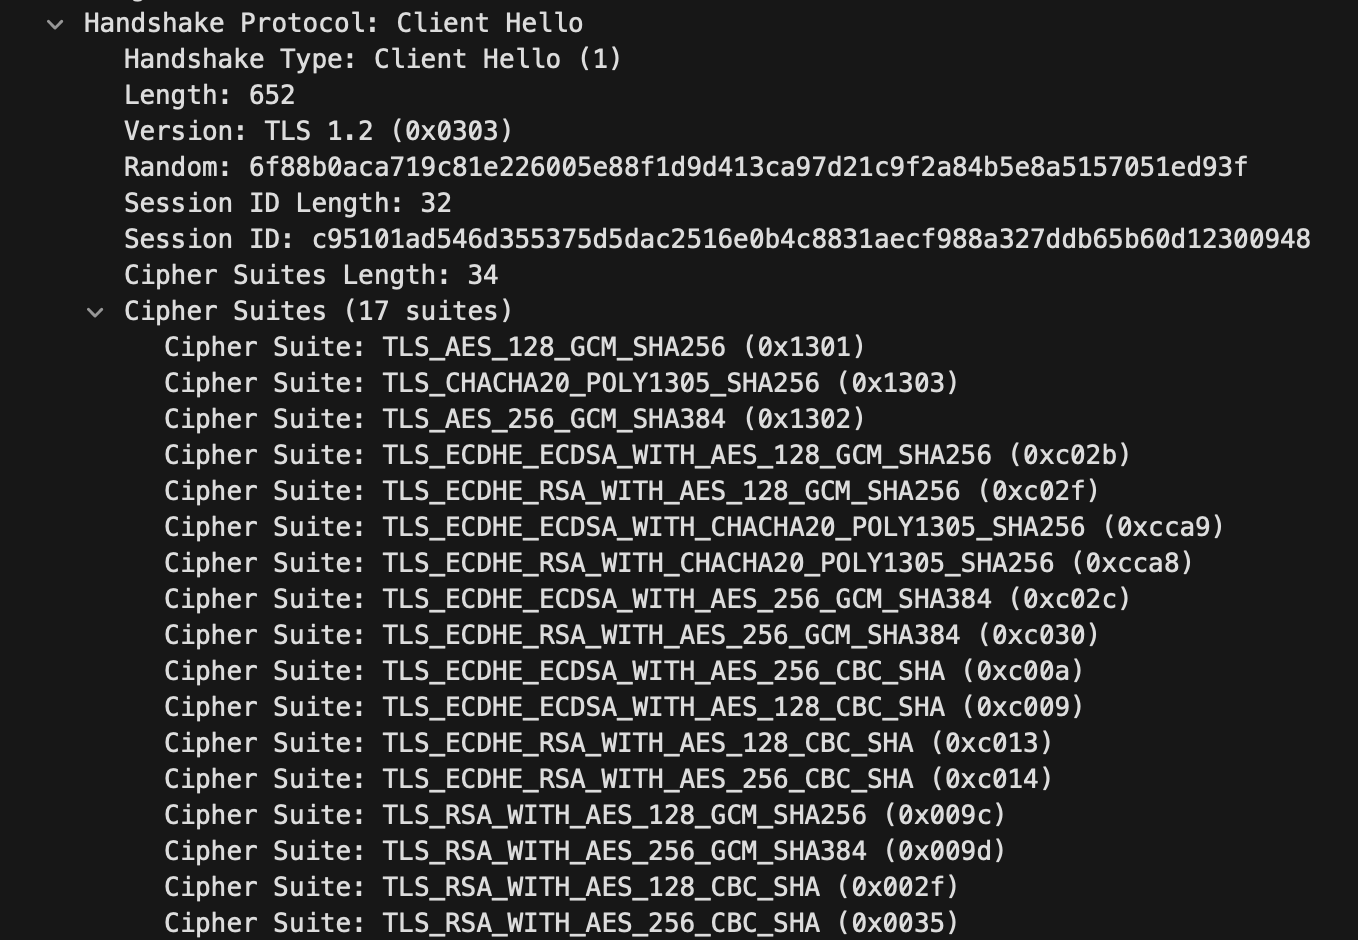
\includegraphics[width=0.7\linewidth]{figures/cipher_suites.png}
    \end{figure}
\end{frame}

\begin{frame}{TLS Handshake: clientHello}
    The \texttt{clientHello} also includes the supported groups for DH or ECDH, and preemptively includes some public keys.
    \begin{figure}
        \centering
        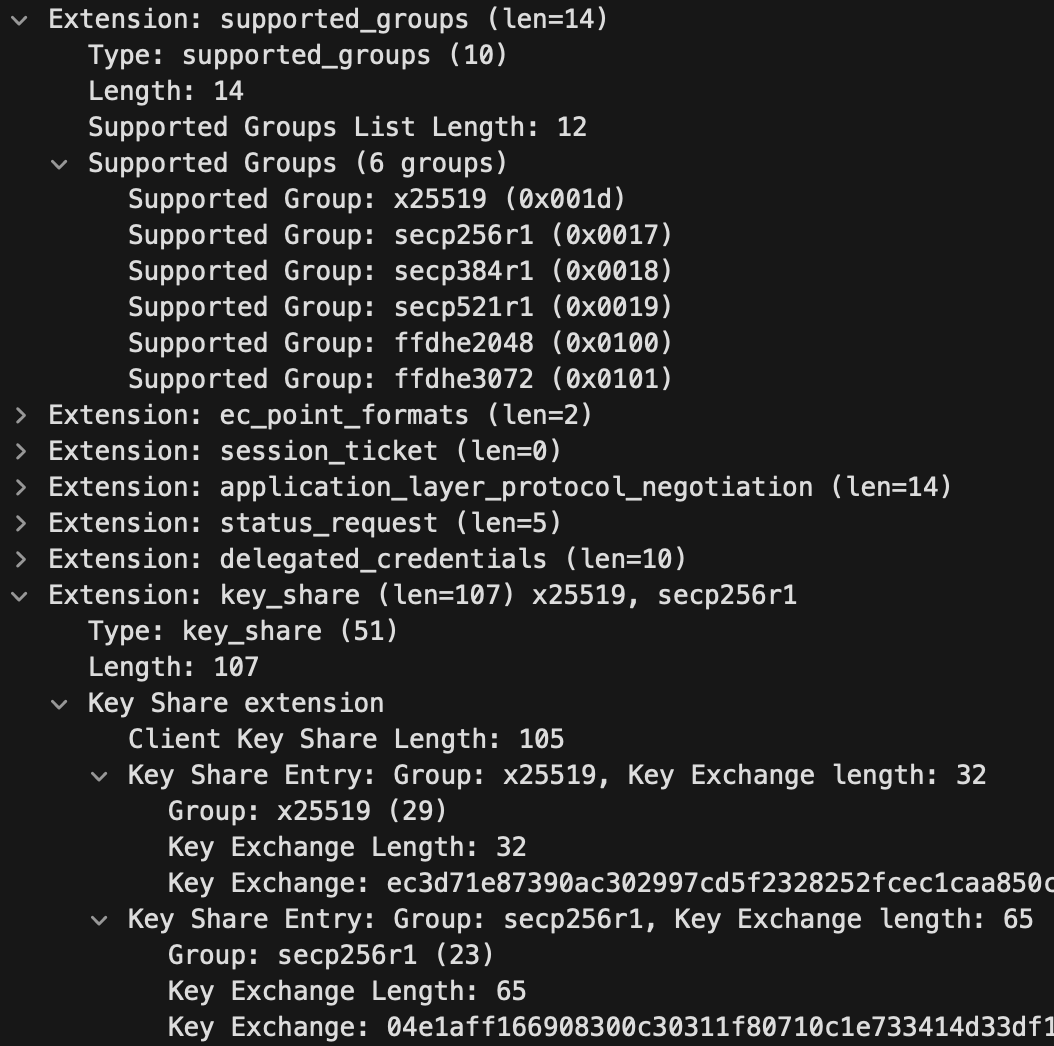
\includegraphics[width=0.7\linewidth]{figures/ch_dh.png}
    \end{figure}
\end{frame}

\begin{frame}{TLS Handshake: serverHello}
    The \texttt{serverHello} responds with the selected cipher suite and their public ECDH x25519 public key.
    \begin{figure}
        \centering
        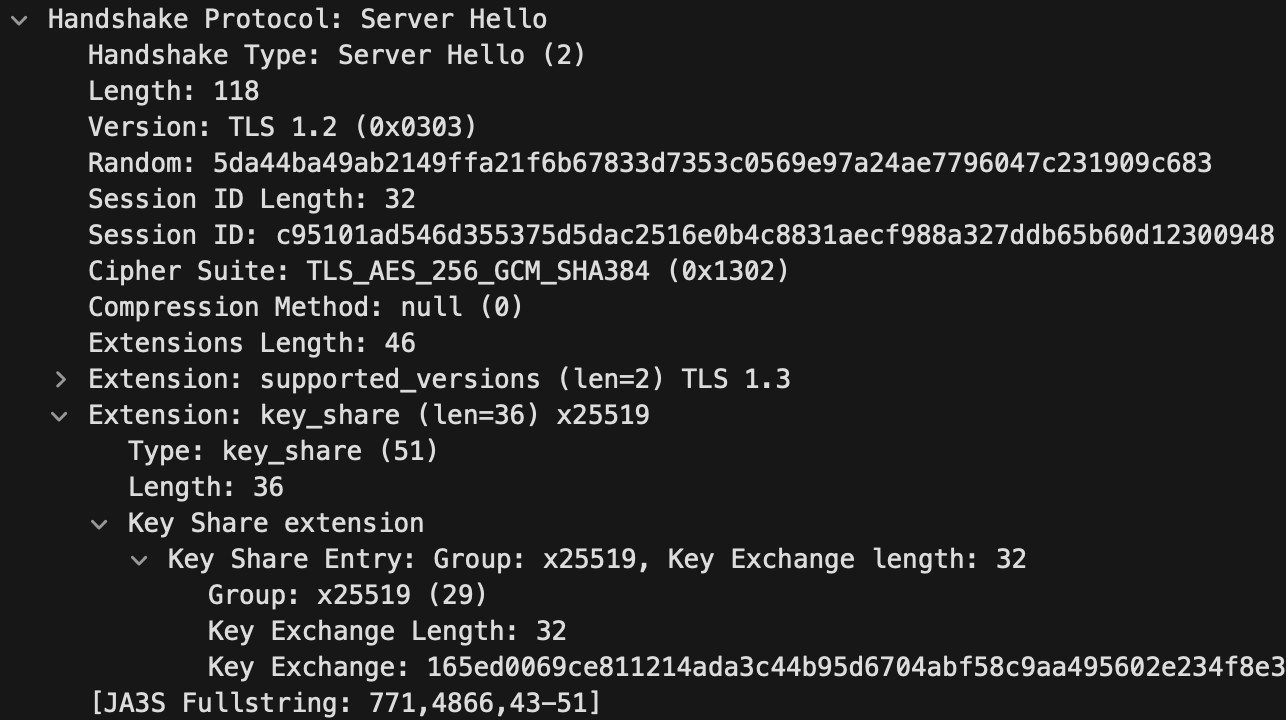
\includegraphics[width=0.9\linewidth]{figures/sh_dh.png}
    \end{figure}

\end{frame}


\begin{frame}{TLS Handshake: Key Schedule}
    Once we have the shared secret established through ECDH on the group x25519, we use this to derive a master key.
    \begin{figure}
        \centering
        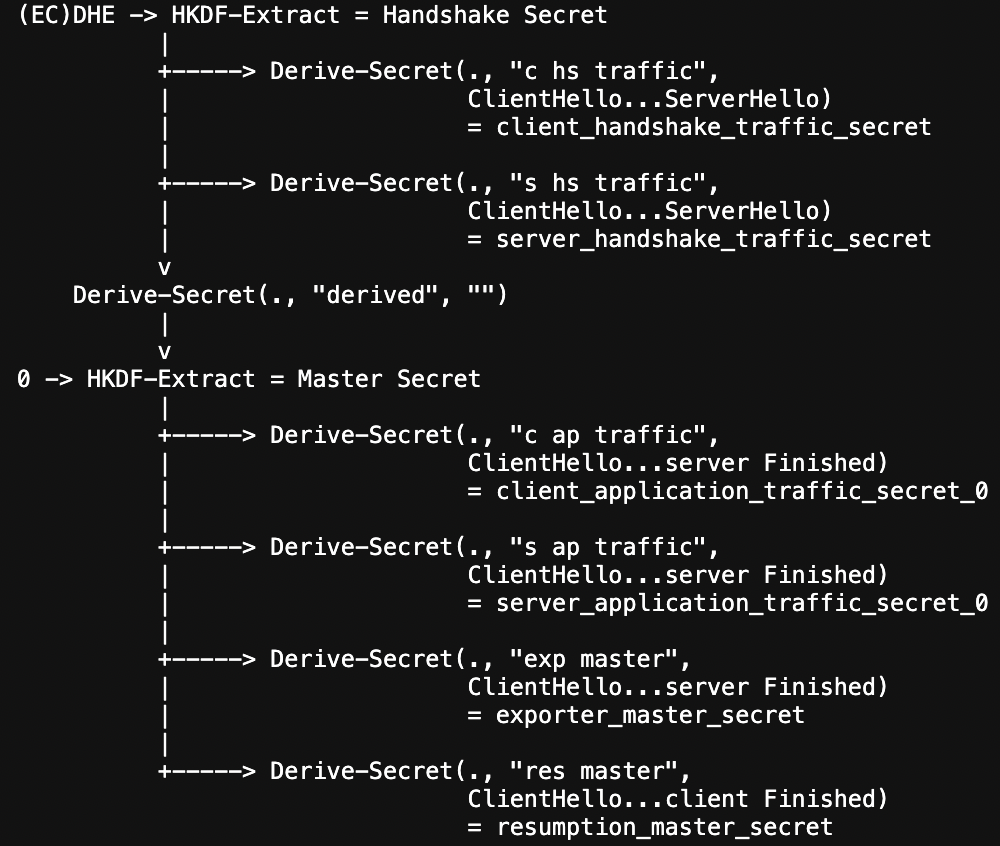
\includegraphics[width=0.7\linewidth]{figures/key_derivation_schedule.png}
    \end{figure}
\end{frame}

\begin{frame}{TLS Handshake: Hash Key Derivation Function HKDF}
    HKDF has two modules, HKDF-Extract, and HKDF-Expand.
    \begin{itemize}
        \item \textbf{HKDF-Extract} takes input key material and an optional salt, and outputs a pseudorandom key (PRK)
        \item \textbf{HKDF-Expand} takes the PRK from the last step, some "info", and a Length, and expands the pseudorandomness of the PRK to the desired length 
    \end{itemize}
\end{frame}

\begin{frame}{TLS Handshake: HKDF-Extract}
    HKDF depends on Hash based Message Authentication Code (HMAC) which is defined as the following:
    \[
        \HMAC()
    \]
    \begin{itemize}
        \item \textbf{HKDF-Extract} takes input key material and an optional salt, and outputs a pseudorandom key (PRK)
        \item \textbf{HKDF-Expand} takes the PRK from the last step, some "info", and a Length, and expands the pseudorandomness of the PRK to the desired length 
    \end{itemize}
\end{frame}

\begin{frame}{Addendum: AES-128-GCM}
    We begin with AES-128. AES-128 is a block cipher, which means that given some 128 bit plaintext and a 128 bit key input, it substitutes and permutes the input and renders ciphertext.

    For messages longer than 128 bits, we can split the messages into 128 bit blocks (with padding), then apply the block cipher in parallel. This is called AES-128-ECB (Electronic Code Book)
\end{frame}
\end{document}